\subsection{KNN Results}

For each movie, one of five CPU usage sequence is selected as test data and the rest four sequences are considered as training data set. 
The length of subsequence varying from 60 seconds to 360 seconds is set and each test and training data is divided based on the subsequence length as described in \ref{sec:knn}.
When dividing sequence data, we adopt a concept of sliding window which moves by 1 step size.
Each data sequence consists of $360$ measurement points, and therefore $(360 - subsequence\_length + 1)$ subsequences are generated from the data sequence. 

After building up test data set and training data set by generating subsequences, we apply KNN method in order to classify each subsequence of test data based on training data set. 
In this experiment, $k$ value is set to 3 for the simplicity.
The accuracy of classification according to the length of subsequence is shown in Figure \ref{fig:experiment_knn}.
The accuracy is low as 46$\%$ when subsequence length is set to 60-second.
However, the accuracy increases up to 88$\%$ when subsequence is set to 180-second.
The experimental result shows that given 10 movies and CPU usage statistics of 150 seconds, our side channel attack correctly predicts which movie a user is watching at the accuracy of higher than 80$\%$.

\begin{figure}[!h]
\centering
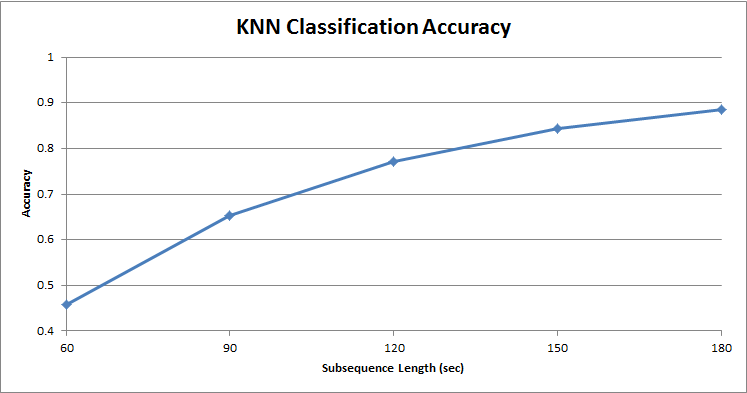
\includegraphics[scale=0.50]{Figures/experiment_knn}
\caption{KNN Classification Accuracy}
\label{fig:experiment_knn}
\vspace{-5mm}
\end{figure}